\section{Introduction}
\subsection{Terminology}
\begin{description}
	\item[Block access] 
		An access to a block of secondary storage. Since accessing secondary storage
		presents itself as the bottleneck in database latency, the time complexity of
		database operations is often represented by the number of block accesses rather
		than the number of RAM operations.
    \item[Data client]
    	A person or party collecting data for the puposes of learning analytics.
    \item[Data subject]
    	A person who contributes data to or is the subject of a learning analytics 
    	application. In the context of the survey tool, this is the person who
    	responds to a survey.
    \item[Learning management system]
	    A content management system, specifically designed for e-learning applications.
	    Examples of LMSs are Moodle and OLAT.
    \item[Learning record store]
    	A database system, possibly including analysis and visualization capabilities, 
	    for storing data of interest to learning analytics applications.
	    In the context of this thesis, LRS particularly refers to a system for storing and analyzing xAPI statements.
    	Examples for LRS systems are the TLA facts engine an HT2Labs's Learning Locker \cite{ht2labs-learninglocker}.
    \item[Survey item]
    	An organizational unit of a survey. In the context of this thesis,
    	a survey item may either be an entire questionnaire, a
    	dimension of a questionnaire or a single question. 
    \item[Tool provider]
	    In the context of LTI, the term \textit{tool provider} is used to describe a
	    system which provides an external tool to an LMS, thereby extending the capabilities of the LMS.
\end{description}

\subsection{The TLA Ecosystem}
    The current efforts of Prof. H. Drachsler's work group are targeted towards the implementation
    of a trusted learning analytics (TLA) infrastructure. This infrastructure will
    provide big data storage and analysis capabilities while complying with the European General
    Data Protection Regulation (GDPR). Data providers present a central part of this infrastructure.
    These data providers are tools used for collecting data and publishing it to
    the TLA facts store, using the xAPI statement format as common data representation (CDR).
    The aim here is not only to create the infrastructure for collecting and analyzing data,
    but also to build an ecosystem of external tools and data providers
    to interface with the TLA core's components.

\subsection{Motivation}
    By no stretch of the imagination are online survey tools a new invention.
    An online search yields dozens of already existing survey platforms, both
    commercial and free to use. Some of the biggest competitors in this business
    are compared in Table \ref{table:competitors}. For most use cases, one
    of the existing solutions will be sufficient. The survey tool described here
    aims at solving a unique challenge not solved by any competitor that the author
    is aware of. This challenge is integration with Moodle and the TLA
    infrastructure for use at the Goethe University in Frankfurt.
    Features needed for this integration are single sign-on, i.e.
    automated authentication of survey participants between Moodle and
    the survey tool, support for embedding via the LTI protocol, 
    as well as support for xAPI as a data exchange protocol.
    These requirements are discussed in greater detail in the Section
    ``Requirements Analysis''. While most survey providers provide single
    sign-on features, these capabilities are generally only provided to enterprise
    customers. Furthermore, only one of the competitors examined in this thesis
    supports CAS as a mechanism for this. None of the competitors
    support data export as xAPI statements out of the box and require either
    manual programming for every survey or data conversion after export. 
    Of the listed competitors, only one supports the LTI protocol for
    embedding the survey into Moodle and the only documentation of this 
    feature is an online video \cite{qualtrics-lti-video}. For these
    reasons, an alternative survey tool was developed.

    %\begin{landscape}
    {\renewcommand{\arraystretch}{1.5}
        \begin{table}
            \begin{tabularx}{1\textwidth}{|l|X|X|X|}
                \hline
                \diagbox{Feature}{Provider} & Google Forms & SurveyMonkey & QuestionPro \\
                \hline 
                SSO & For managed accounts in G-Suite via SAML and LDAP \cite{googleforms-sso}
                    & Supported, but further information is only provided to potential customers. \cite{surveymonkey-sso}
                    & Through SAML and HMAC-SHA1 \cite{questionpro-sso}
                    \\
                xAPI & Not supported, but has limited support for programmable event handlers. \cite{googleforms-webhooks}
                     & Not supported, but supports polling of survey results through an API. \cite{surveymonkey-api}
                     & Not supported, but has support for web hooks. \cite{questionpro-webhooks}
                     \\
                LTI & Unsupported 
                    & Unsupported 
                    & Unsupported
                    \\
                \hline
            \end{tabularx}
            \vskip 1em
            \begin{tabularx}{1\textwidth}{|l|X|X|}
                \hline
                \diagbox{Feature}{Provider} & qualtrics & survey gizmo \\
                \hline 
                SSO 
                    & Through CAS, LDAP or SAML \cite{qualtrics-sso}
                    & Through SAML \cite{surveygizmo-sso} \cite{surveygizmo-sso2}
                    \\
                xAPI 
                     & Not supported, but supports polling of survey results through an API. \cite{qualtrics-api}
                     & Not supported, but has limited support for web hooks. \cite{surveygizmo-webhooks}
                     \\
                LTI
                    & Alledged experimental support, no official documentation exists. 
                    & Unsupported
                    \\
                \hline
            \end{tabularx}
            \caption{Comparison of survey providers}
            \label{table:competitors}
        \end{table}
    }
    %\end{landscape}


\subsection{Previous Work}
    As part of the computational humanities seminar, conducted by \profhd in the 2017/18 winter semester, Hannes Leutloff
    and I were tasked to digitize the evaluation framework for learning analytics (EFLA) \cite{efla} and to
    develop an online platform where the survey could be taken.

    \begin{figure}
        \centering
        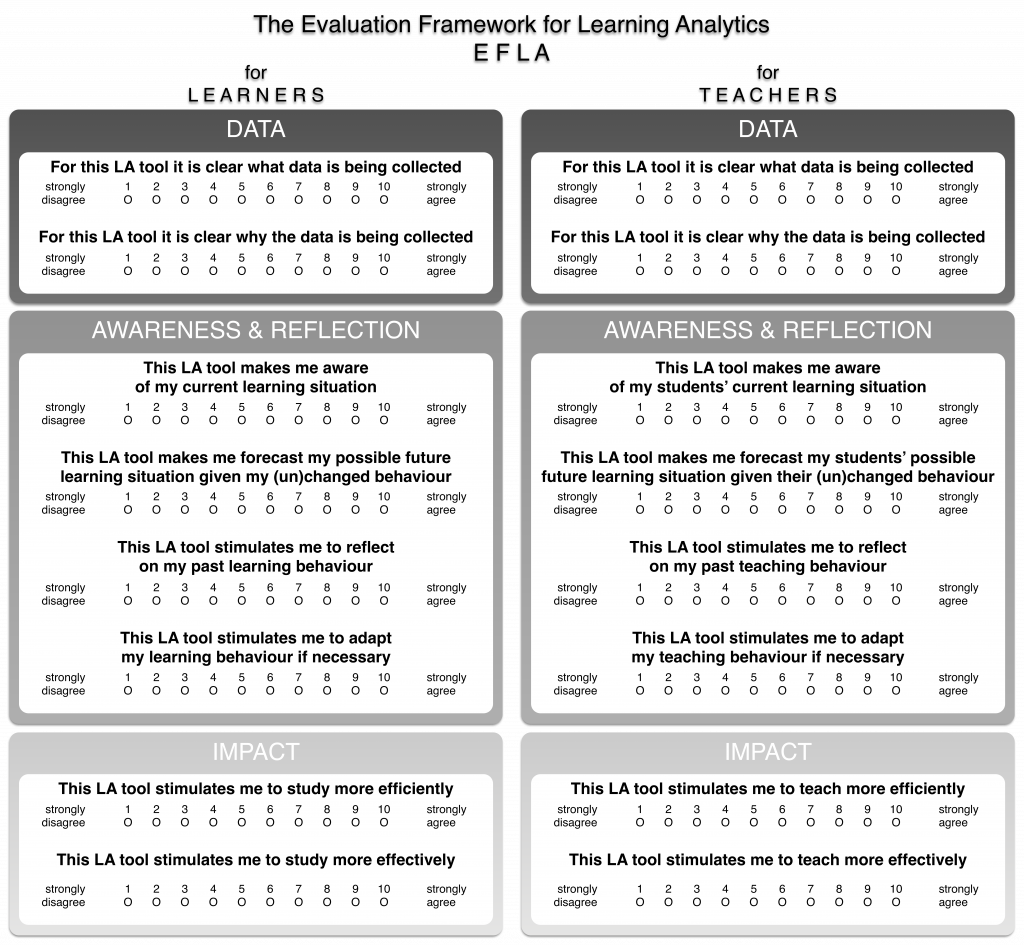
\includegraphics[width=\textwidth]{EFLA--greyscale}
        \caption{Template for the EFLA survey \cite{efla-website}}
        \label{fig:efla-template}
    \end{figure}

   The result is an online survey platform, where surveys similar to the EFLA can be created
   and hosted. While it is possible to create arbitrary survey items, some restrictions
   specific to the EFLA use-case apply (for a full list of features see Table \ref{table:v1-features}).
   The original version of the survey tool is written in Python 3 and JavaScript for the server
   and user interface respectively. To be able to re-use code, the choice of language did not
   change with the new version.
   

   \begin{figure}
       \begin{tabularx}{\textwidth}{|l|X|}
            \hline
            Feature & Description \\
            \hline \hline
            Editable surveys & Edit titles, question texts and colors.\\
            Export to CSV & Export all results of a questionnaire to as CSV file\\
            Challenges & Validate data subject's email addresses. 
            White- and Blacklist email addresses. Protect surveys by password.\\
            Internationalisation & Survey items may have multiple translations.\\
            User accounts & Users may sign up and host surveys.\\
            Template surveys & Choose from a fixed set of template surveys.\\
            Visualization & View survey results as a box plot.\\
            \hline
       \end{tabularx}
       \caption{Features of the previous version of the survey tool}
       \label{table:v1-features}
   \end{figure}

   \subsubsection{Data Model}

   \begin{figure}[H]
        \centering
        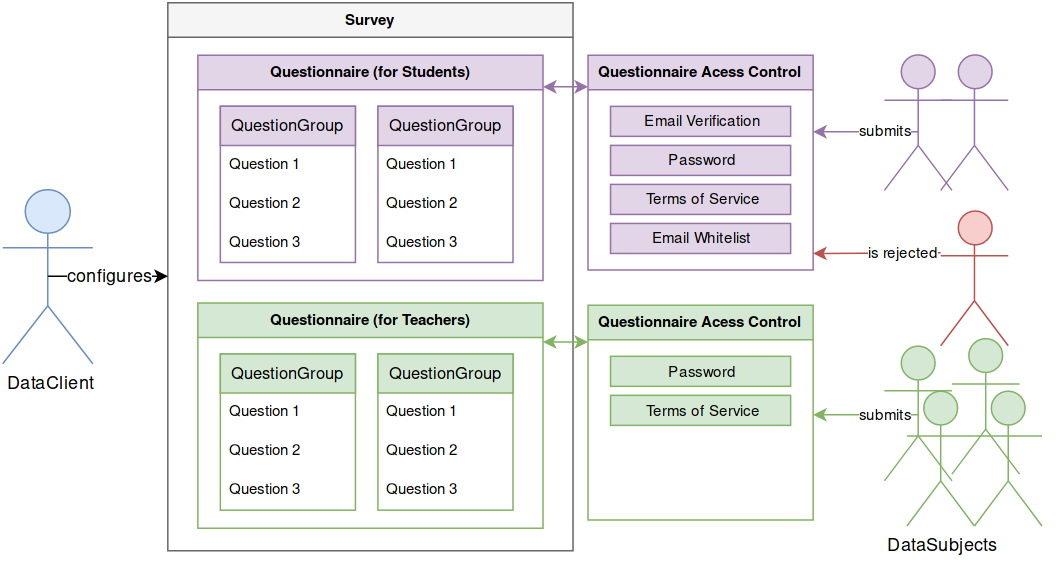
\includegraphics[width=\textwidth]{v1-model}
        \caption{Data model of the previous version}
        \label{fig:v1-data-model}
    \end{figure}

    \begin{wrapfigure}{o}{.5\textwidth}
        \centering
        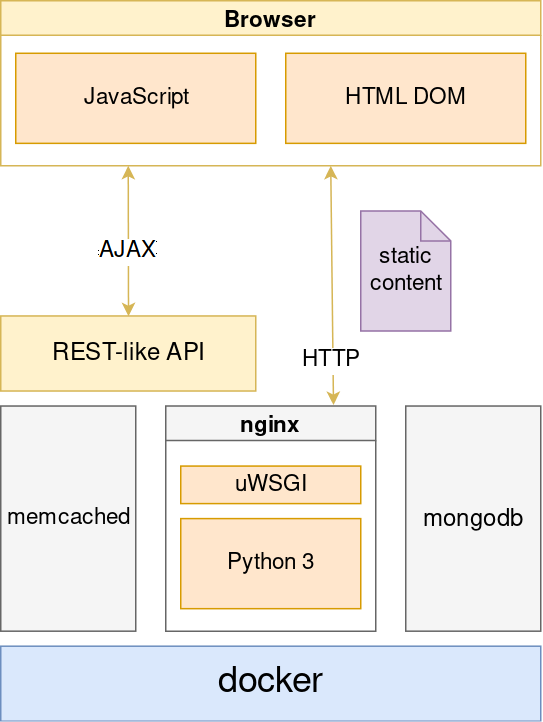
\includegraphics[width=0.4\textwidth]{v1-stack}
        \caption{Architecture overview of the previous version}
        \label{fig:v1-stack}
    \end{wrapfigure}

    The data model for the previous version is closely coupled to the specific needs of the
    EFLA survey, where a single survey consists of two questionnaires, targeting
    learners and teachers respectively.
    Each questionnaire controls the submission right of data subjects by its own set of access 
    control modules, so that audience groups can be differentiated.
    Each questionnaire contains one or more question groups, which consists of
    one or more questions.

    \subsubsection{Architecture}
        The architecture for the previous version follows a simple client-server paradigm, where
        a web browser assumes the role of the client. The server software consists of an
        application server, responding to API requests, a database and an in-memory
        key-value store for storing session data. There are two different user interfaces,
        one for data clients and one for data subjects. The data subjects' user interface
        is the page, where the survey is filled out and submitted. This page is rendered
        on the server using a templating engine and sent to the browser as a static HTML document.
        The user interface for data clients presents the user with an editor, where survey content
        can be created and modified. This user interface is realized as a one-page
        JavaScript application and was developed by Hannes Leutloff. Deployment is handled through
        Docker, with the help of the docker-compose tool.

\subsection{Goal}
    The goal of this thesis is to extend the functionality of the already existing
    survey tool and to contribute to the TLA ecosystem by integrating the
    survey tool as a data provider. In this thesis, the overall structure of the 
    survey platform and the server-side software stack, designed and developed 
    by Noah Hummel, is discussed. Implementational details are discussed only 
    if they are central to the workings of the software, or solve a particular 
    conceptual challenge. As the user interface was designed and mainly developed by 
    Hannes Leutloff, it is therefore not discussed here.

\subsection{Additional Contents}
\subsubsection{Source Code}
    The source code for this project is maintained at GitHub and can be found at
    \url{https://github.com/yeldiRium/st3k101}.
    The version submitted as part of this thesis is version \inline{3.1.0-beta}, 
    which can be accessed at \url{http://bit.ly/xapi-probe-3}. There, the
    source code is available as a zip-compressed archive. The reader may
    prove the authenticity of the release by calculating the archive's
    SHA-1 hash sum. \\
     
    \inline{st3k101-3.1.0-beta.tar.gz: 1f1ce2727378713bedaaf801eaa5a4d2004f9d62}
     
    \inline{st3k101-3.1.0-beta.zip: 5a38cc5e485c249c9a215b0dd997fac77cc6c595}\\[1em]

\subsubsection{Documentation}
    The source code itself is documented using docstrings and comments.
    The project's \inline{README} file is the central point of access
    for information on deployment, dependencies and development
    setup.

\subsubsection{API Reference}
    The API reference for the \inline{backend} service can be accessed
    at \url{http://bit.ly/xapi-probe-api-v6}. This version exists
    for reference only and will not be updated.